\section{Supplementary experimental results}
\label{sec:supp-experiment}%

Due to limited space, we considered the surrogate loss without the zero-one loss in Figure~\ref{fig:illustration}. Here, we include the zero-one loss and show the extended version of Figure~\ref{fig:illustration} in Figure~\ref{fig:more-illustration}. In general, the curves of risks w.r.t.\ $\ell_{01}$ look quite similar to (but less smooth than) those w.r.t.\ $\ellsig$. Therefore, the curves of risks w.r.t.\ $\ellsig$ are more visually appealing as the illustrative experimental results.

\begin{figure*}[h]
  {\centering
    \subcaptionbox{Linear model, risks w.r.t.\ $\ellsig$}
    {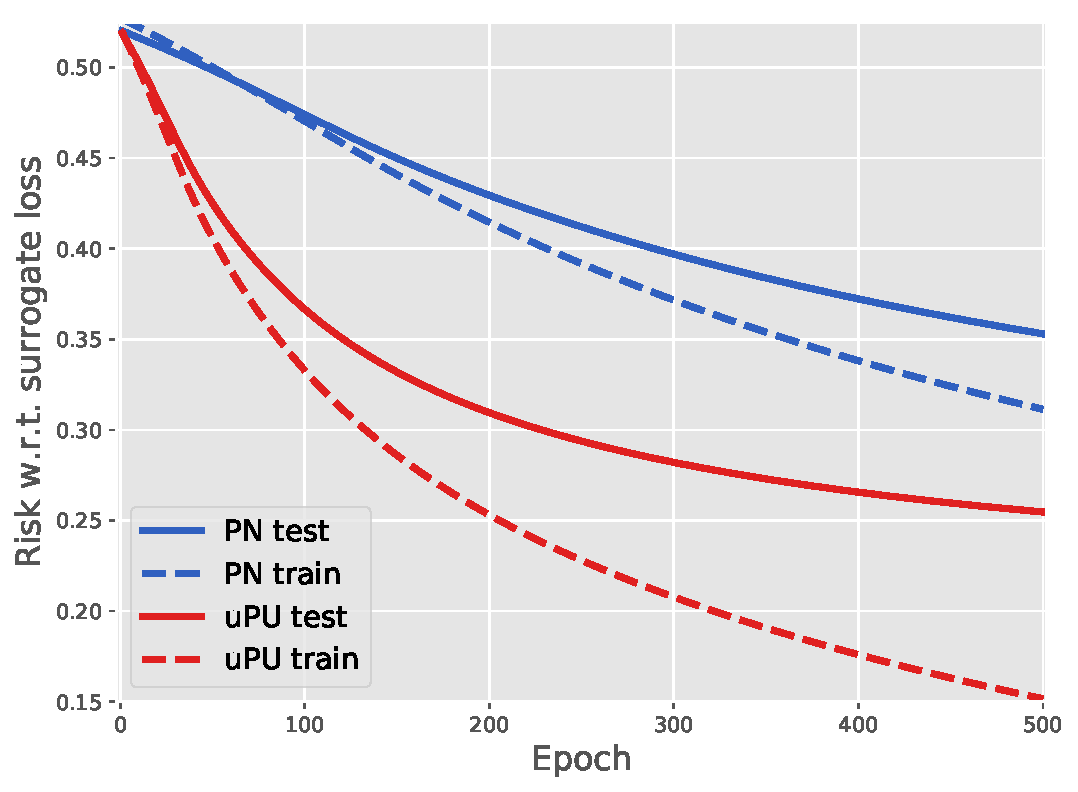
\includegraphics[width=0.5\textwidth]{illustration_surrogate_linear}}%
    \subcaptionbox{Linear model, risks w.r.t.\ $\ell_{01}$}
    {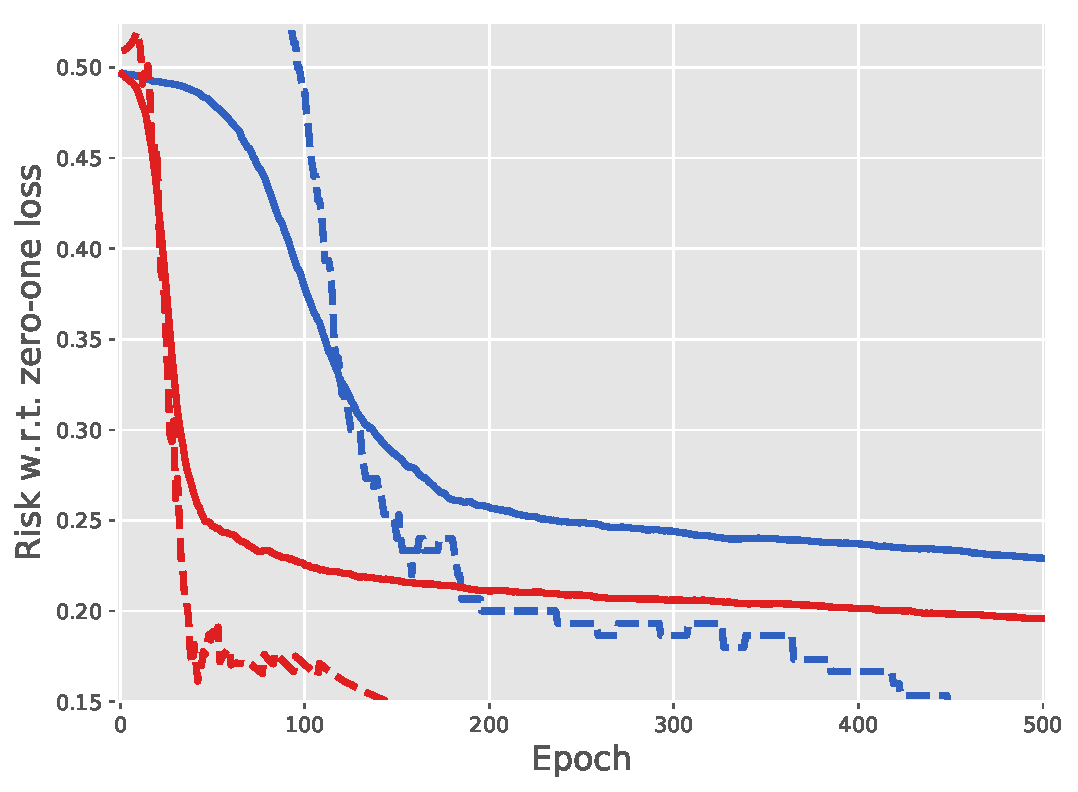
\includegraphics[width=0.5\textwidth]{illustration_zero-one_linear}}\\
    \subcaptionbox{MLP, risks w.r.t.\ $\ellsig$}
    {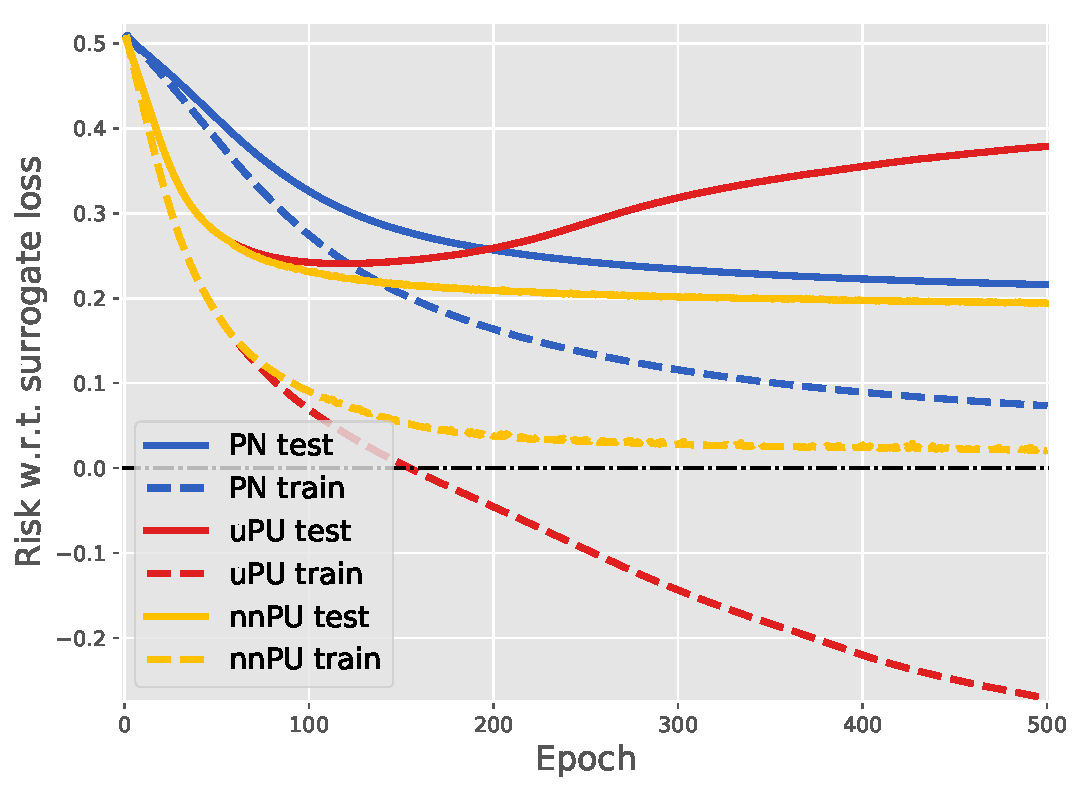
\includegraphics[width=0.5\textwidth]{illustration_surrogate_mlp}}%
    \subcaptionbox{MLP, risks w.r.t.\ $\ell_{01}$}
    {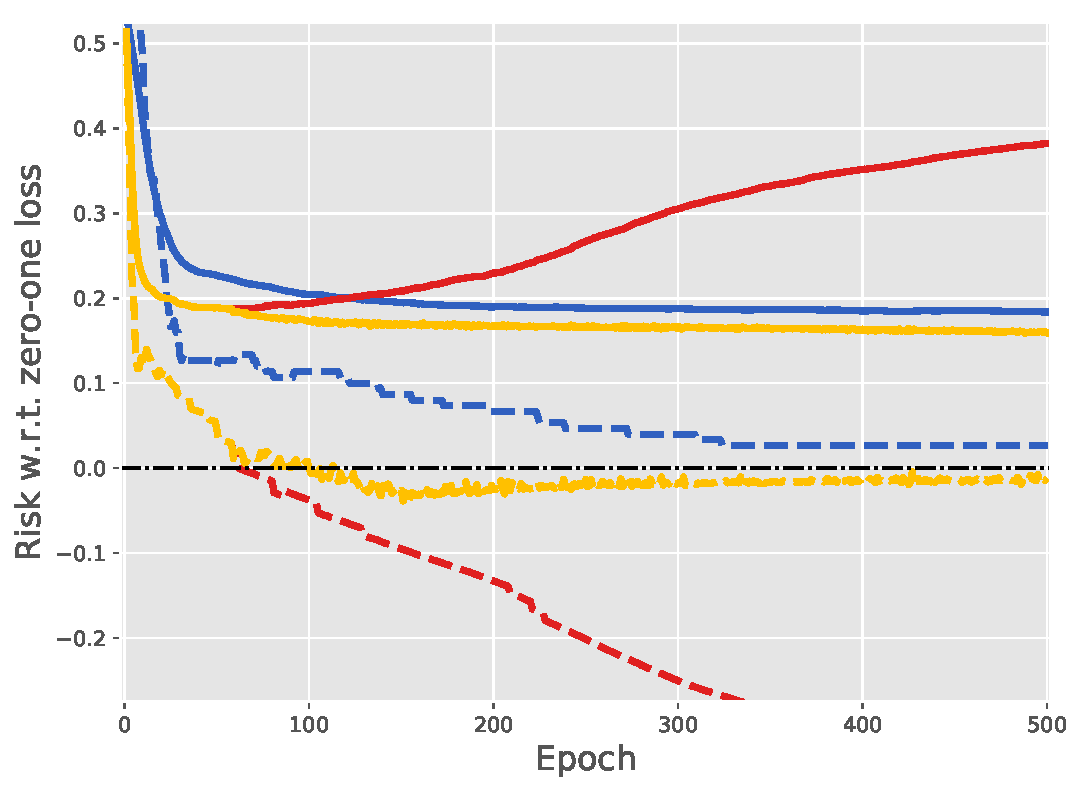
\includegraphics[width=0.5\textwidth]{illustration_zero-one_mlp}}}
  \caption{The extended version of Figure~\ref{fig:illustration}.}
  \label{fig:more-illustration}
\end{figure*}
